\newcommand{\lecture}{Network Performance and Modelling\\
FS2013} 
\newcommand{\serieNumber}{Practical Exercise\\ Final Report} 
\newcommand{\authorsOfSerie}{Steve Aschwanden 05-480-686\\ Tobias Schmid 07-909-294}


\documentclass[a4paper]{article} 
\usepackage{documentstyle}

\begin{document} 
%Header %
\pagestyle{fancy} %eigener Seitenstil
\fancyhf{} %alle Kopf- und Fußzeilenfelder bereinigen
\fancyhead[L]{\lecture} %Kopfzeile links
\fancyhead[C]{\serieNumber} %zentrierte Kopfzeile
\fancyhead[R]{\authorsOfSerie} %Kopfzeile rechts
\renewcommand{\headrulewidth}{0.4pt} %obere Trennlinie
\fancyfoot[C]{\thepage} %Seitennummer
\renewcommand{\footrulewidth}{0.4pt} %untere Trennlinie

 

\begin{center}
	\huge{Comparison of TCP and SCTP transport protocols over wireless multi-hop networks}
\end{center}

\begin{abstract}
The Stream Control Transmission Protocol (SCTP) was defined, about twenty years after TCP and UDP, in 2000 by the Internet Engineering Task Force (IETF). They combined the best practices from both older protocols to create a message-based, multi-streamed transport protocol. There are papers \cite{sctp_vs_tcp}\cite{sctp_vs_tcp2} which shows the improvements of the SCTP with the usage of HTTP over the internet. In this paper the behaviour of the TCP and SCTP in a wireless multi-hop network environment is compared. For this the OMNeT++ network simulation framework \cite{omnetpp} has been used. The hops are in motion (different speeds) and use the proactive OLSR protocol to transmit data over a wide open field (500m x 500m) without obstacles like mountains or buildings. In the first part the reader is introduced into some technical topics for a better understanding of the used technologies. The simulation setting and the corresponding results are part of the mid section. At the end of the document a conclusion of the project with a summary of the observations is made.
\end{abstract}

\tableofcontents
\pagebreak

\section{Introduction}

\subsection{Transmission Control Protocol}

The Transmission Control Protocol (TCP) is besides the User Datagram Protocol (UDP) one of the core protocols of the Internet Protocol suite (IP) which has been developed between the mid-seventies and the early-eighties of the 20th century.\\
TCP provides connection oriented data-transfer with the following key features:
\begin{itemize}
	\item Ordered data transfer
	\item Retransmission of lost packets
	\item Error-free data transfer 
	\item Flow control 
	\item Congestion control
\end{itemize}
Since TCP is the most common used transport protocol it is assumed that the reader is familiar with the operation of the Protocol. Because of that the focus of the introduction lies on the less common protocols used in this simulation scenario.

\subsection{Stream Control Transmission Protocol}
Stream Control Transmission Protocol (SCTP) is a reliable, message oriented transport protocol that provides new services and features for IP communication. For the past twenty years, reliable communication service has been provided by TCP, unreliable by UDP. So, what has brought about the addition of a third protocol to the IP suite of protocols? Many of the features found in TCP and UDP can also be found in SCTP (see Table \ref{tab_sctp_features}).
\begin{table}[H]
	\centering
	\begin{tabular}{ | l | r | r | r | }
		\hline
		Service/Features & SCTP & TCP & UDP \\ \hline \hline
		Message-Oriented & yes & no & yes \\ \hline
		Byte-Oriented & no & yes & no \\ \hline
		Connection-Oriented & yes & yes & no \\ \hline
		Full Duplex & yes & yes & yes \\ \hline
		Reliable data transfer & yes & yes & no \\ \hline
		Partially-Reliable data transfer & opt & no & no \\ \hline
		Ordered data delivery & yes & yes & no \\ \hline
		Unordered delivery & yes & no & yes \\ \hline
		Flow control & yes & yes & no \\ \hline
		Congestion Control & yes & yes & no \\ \hline
		Selective Acknowledgements & yes & opt & no \\ \hline
		Multistreaming & yes & no & no \\ \hline
		Multihoming & yes & no & no \\ \hline
		Dynamic Multihoming & opt & no & no \\ \hline
		SYN flooding attack prevention & yes & no & n/a \\ \hline
		Allows half-closed state & no & yes & n/a \\ \hline
		Reach-ability check & yes & opt & no \\ \hline
	\end{tabular}
	\caption{Feature comparison}
	\label{tab_sctp_features}
\end{table}



\subsubsection{Key Benefits}
SCTP improves upon TCP and UDP by integrating components of each. But the designers of SCTP did not stop there. There have been two new concepts added: multi-homing and multi-streaming.

\paragraph{Multi-homing}
SCTP was designed to handle the signalling of telecommunications over IP. Since  telecommunications are very susceptible to time delays, every millisecond counts. Multi-homing enables systems that have multiple interfaces, for redundancy, to use one over the other without having to wait. Within SCTP one interface is established as the primary and the rest become secondary. If the primary should fail for whatever reason, a secondary is selected and utilized. When the primary becomes available again, the communications can be transferred back without the application being aware there was an issue. While establishing the connections, the primary and secondary interfaces are checked and monitored using a heartbeat/heartbeat  acknowledgement process that validates addresses, and maintains a Round Trip Time (RTT) calculation for each address. The RTT can indicate that the primary is slower than a secondary and allow for the communications to migrate to the secondary interface.

\paragraph{Multi-streaming}
Using TCP, only one single data stream is allowed per connection. All of the information must be passed through that one stream. SCTP allows multiple simultaneous data streams within a connection or association. Each message sent to a data stream can have a different final destination, but each must maintain message boundaries. For example, systems cannot send parts of the same message through different streams; one message must go through one stream. When running an ordered data delivery system, if one of the packets is out of order or missing, the stream is blocked pending resolution to the order. This is called “Head-of-Line Blocking.” With the use of multi-streams, only the stream that is affected would be blocked; the other streams would continue to flow. By using multi-streaming with SCTP, the issue with web browsers only having the ability to handle two simultaneous connections goes away. The client or the web server could immediately open additional streams and send pictures, text, etc. through each stream, reducing overall latency. This could also reduce overhead that servers often incur with the numerous separate connections required to fulfil a request.

\paragraph{Selective acknowledgements}
In standard TCP, every message, or packet of information must be accounted for, resent as necessary, and processed in the order they were sent. SCTP has the ability to selectively acknowledge receipt of missing, disordered, or duplicated messages. Due to the nature of telecommunications most applications would end up discarding any unsynchronized messages. Therefore, the need to send and receive the information is forgone. This would mean that a portion of a word, a portion of a video, or a piece of the whiteboard refresh would be skipped over. The applications and users may notice a slight skip in the voice, video, or refresh. This is referred to as jitter within the telecommunications world and a small amount of jitter is often preferred to having the packet resent and reprocessed which would double the amount of jitter, usually making it more noticeable to the users.

\paragraph{Unordered data delivery}
Due to the very nature of networks not all packets may travel across the exact same path. If there is a time-delay using one path over another, the original messages could be out of order when received. Unordered data delivery allows for this instance and can correct the issue by reordering the messages correctly. Using TCP’s reliable data transfer feature requires that packets be processed in order. If one is missing or out of order, the packet must be reordered before processing can continue. SCTP allows for unordered data delivery and since it has multiple streams, only the one affected is temporarily blocked.

\subsection{Optimized Link State Protocol}
Optimized Link State Protocol (OLSR) is a proactive routing protocol, so the routes are always immediately available when needed. OLSR is an optimization version of a pure link state protocol. The topological changes cause the flooding of the topological information to all available hosts in the network. To reduce the possible overhead in the network protocol uses Multipoint Relays (MPR). The idea of MPR is to reduce flooding of broadcasts by reducing the same broadcast in some regions in the network.

\subsubsection{Control messages}
OLSR uses two kinds of the control messages: Hello and Topology Control (TC). Hello messages are used for finding the information about the link status and the host’s neighbours. With the Hello message the Multipoint Relay (MPR) Selector set is constructed which describes which neighbours has chosen this host to act as MPR and from this information the host can calculate its own set of the MPRs. The Hello messages are sent only one hop away but the TC messages are broadcasted throughout the entire network. TC messages are used for broadcasting information about own advertised neighbours which includes at least the MPR Selector list. The TC messages are broadcasted periodically and only the MPR hosts can forward the TC messages.
There is also Multiple Interface Declaration (MID) messages which are used for informing other host that the announcing host can have multiple OLSR interface addresses. The MID message is broadcasted throughout the entire network only by MPRs. There is also a “Host and Network Association” (HNA) message which provides the external routing information by giving the possibility for routing to the external addresses. The HNA message provides information about the network- and the netmask addresses, so that OLSR host can consider that the announcing host can act as a gateway to the announcing set of addresses. The HNA is considered as a generalized version of the TC message with only difference that the TC message can inform about route cancelling while HNA message information is removed only after expiration time.

\subsubsection{Multipoint relays}
The Multipoint Relays (MPR) is the key idea behind the OLSR protocol to reduce the information exchange overhead. Instead of pure flooding the OLSR uses MPR to reduce the number of the host which broadcasts the information throughout the network. The MPR is a host’s one hop neighbour which may forward its messages. The MPR set of host is kept small in order for the protocol to
be efficient. In OLSR only the MPRs can forward the data throughout the network. Each host must have the information about the symmetric one hop and two hop neighbours in order to calculate the
optimal MPR set. The two hop neighbours are found from the Hello message because each Hello message contains all the hosts’ neighbours. Selecting the minimum number of the one hop neighbours which covers all the two hop neighbours is the goal of the MPR selection algorithm.
Also each host has the Multipoint Relay Selector set, which indicates which hosts has selected the current host to act as a MPR. When the host gets a new broadcast message, which is need to be spread throughout the network and the message’s sender interface address is in the MPR Selector set, then the host must forward the message. Due to the possible changes in the ad hoc network, the MPR Selectors sets are updated continuously using Hello messages.

\subsubsection{Advantage}
OLSR is also a flat routing protocol, it does not need central administrative system to handle its routing process. The proactive characteristic of the protocol provides that the protocol has all the routing information to all participated hosts in the network. However, as a drawback OLSR
protocol needs that each host periodic sends the updated topology information throughout the entire network, this increase the protocols bandwidth usage. But the flooding is minimised by the MPRs, which are only allowed to forward the topological messages.

\pagebreak
\section{Simulation}

\subsection{Objectives}
OMNeT++ simulation based comparison of the TCP and SCTP transport protocols with respect to performance in wireless multihop networks. Modelling of a point-to-point connection with permanent changing routes due to various moving ad hoc network devices. Simulating an open battlefield area where only free-space loss influences the wireless propagation. Focus the influence of changing routes due to mobility on the announced transport protocols considering various metrics.

\subsection{Scenario}
An important message including maps and pictures has to be transmitted from the army command center (server) at the outer left center of the battlefield to a special force unit (client) at the outer right center of the battlefield (see Figure \ref{fig:topology}). Due to war actions the wired connections are broken and the satellite base station has been destroyed by the enemy. The armed forces only have the possibilities of building an ad hoc wireless network between different squads of their troops. They build network based on the moving velocity of the available squads. There are various troop genres with different average velocities and rate of turn:
\begin{itemize}
	\item Infantry (5 km/h), fast turning
	\item Jeeps (5 - 30 km/h), fast turning
	\item Tanks (5 - 30 km/h), medium turning
\end{itemize}		
Each squad / vehicle has only one wireless device which acts as network routing hop. Tested networks will only be built by equal troop genres to avoid mixed moving parameters.

\subsection{Experiment design}
\subsubsection{Topology}
In this subsection the technical view of the used topology is introduced. Information proposed in the scenario are specified in a more proper form. The following graphic shows the topology used in the simulation. The network consists of two stationary entities with client and server roles. These stationary devices are interconnected over 10 to 15 moving wireless ad hoc devices building a wireless multihop link in between.
\begin{figure}[H]
	\centering
	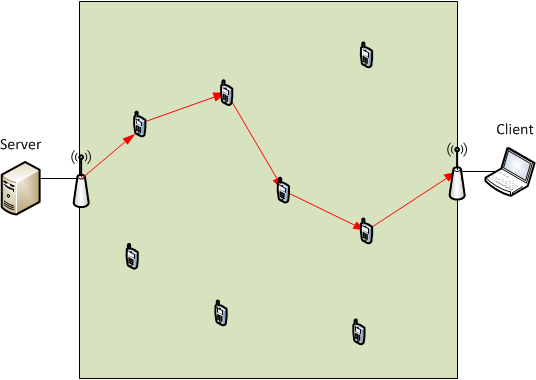
\includegraphics[width=0.5\textwidth]{imgs/Topology}
	\caption{Network Topology}
	\label{fig:topology}
\end{figure}
The following list collects the exact specifications:
\begin{itemize}
	\item Area: Square, 500m x 500m, Free-Space loss
	\item Number of moving devices: 10
	\item Number of stationary devices: 2
	\item Moving speed of mobile devices: 5, 10, 20, 30, 70 km/h
	\item Energy management of mobile devices: Will not be considered
	\item Movement: Random Walk, change of direction with different turning speeds
	\item IEEE802.11a wireless ad hoc network
	\begin{itemize}
		\item Carrier frequency: 2.4 GHz band
		\item Base-Bitrate: 6Mbps
		\item Max-Bitrate: 54Mbps
		\item Transmitter power: 4.5mW
		\item Path loss coefficient: 2 (free space)
	\end{itemize}
	\item Ad hoc routing protocol: OLSR
	\item Traffic modelling: 
	\begin{itemize}
		\item TCP: Single session data transfer of 400MiB
		\item SCTP: Single session data transfer with 1-5 associated streams 
	\end{itemize}
\end{itemize}			
\subsubsection{Simulation}
The simulation runtime was 200 seconds. The simulation time limits the maximal covered walk of a mobile node which is necessary because of the limited area.
\subsubsection{Metrics}
For the comparison of the two transport protocols the following metrics have been used:
\begin{itemize}
	\item Throughput: The average number of bits delivered over a communication channel within a certain amount of time. This metric has the unit bits per second (bps)
	\item Loss rate: The ratio of number of packets which did not reach the destination over the number of all transmitted packets
	\item Round trip time (RTT): The time between sending a packet and the arrival of the corresponding acknowledgement from the server
	\item ACK overhead: The additional number of the control messages sent by the TCP protocol compared to the number of message sent by the SCTP protocol.
\end{itemize}			
\subsubsection{Parameters}
In the discussed simulation the following parameters have been used to show the different behaviour of the transport protocols:
\begin{itemize}
% TODO results are not the average of these three runs but we can tell that it is like this... ;-)
%	\item Number of Test Runs: 3
	\item Type of transport protocol
	\begin{itemize}
		\item Stream Control Transmission Protocol
		\begin{itemize}
			\item Number of streams (1-5)
		\end{itemize}
    	\item Transmission Control Protocol (Standard implementation of INET framework)
	\end{itemize}
	\item Moving speed of mobile devices
	\begin{itemize}
		\item Speed (5, 10, 20, 30, 70 km/h)
	\end{itemize}
\end{itemize}	

% TODO remove this lines
The suggested number of streams is only a first estimation. If we can’t see distinguished results during the simulation process, we will have the possibility to change these numbers.
\subsection{Results}
\subsubsection{Expected results}
In this section a prediction about the results of the discussed simulation approach is made.

\paragraph{Throughput}
The TCP should have a slightly higher throughput than SCTP if only one stream is used. Because the SCTP can not bring in his strength (multiple streams, message oriented). Increasing the number of streams while having a small loss rate (e.g. slow velocity) is not enough to beat the performance of TCP. But if there are losses (e.g. high velocity), SCTP has the mechanism to achieve a higher throughput.
\paragraph{Loss rate}
A small moving speed of the mobile devices should result in a small loss rate. This behaviour is expected because the routing needs enough time to find a new route to the destination. If the velocity will be increased, then the loss rate increases too. The type of the transport protocol should have no influence to the loss rate.
\paragraph{Round trip time (RTT)}
Using only one stream of the SCTP will not reduce the RTT and therefore the TCP will have a smaller one. But if multiple stream are used then the SCTP should reduce this metric significantly. The parallelism could be one reason to explain this. Generally, a higher velocity of the devices results in higher RTT (OLSR has to find new routes faster).
\paragraph{ACK Overhead}
Increasing velocity will cause an increasing ACK overhead of TCP because packets are dropped and have to be retransmitted. The number of packet requests of SCTP increases with a higher number of streams and increasing velocity because of packet loss.

\subsubsection{Measured results}

\paragraph{Throughput}

First of all the throughput of TCP and STCP have been compared with different movement velocities. 

\begin{figure}[H]
	\centering
	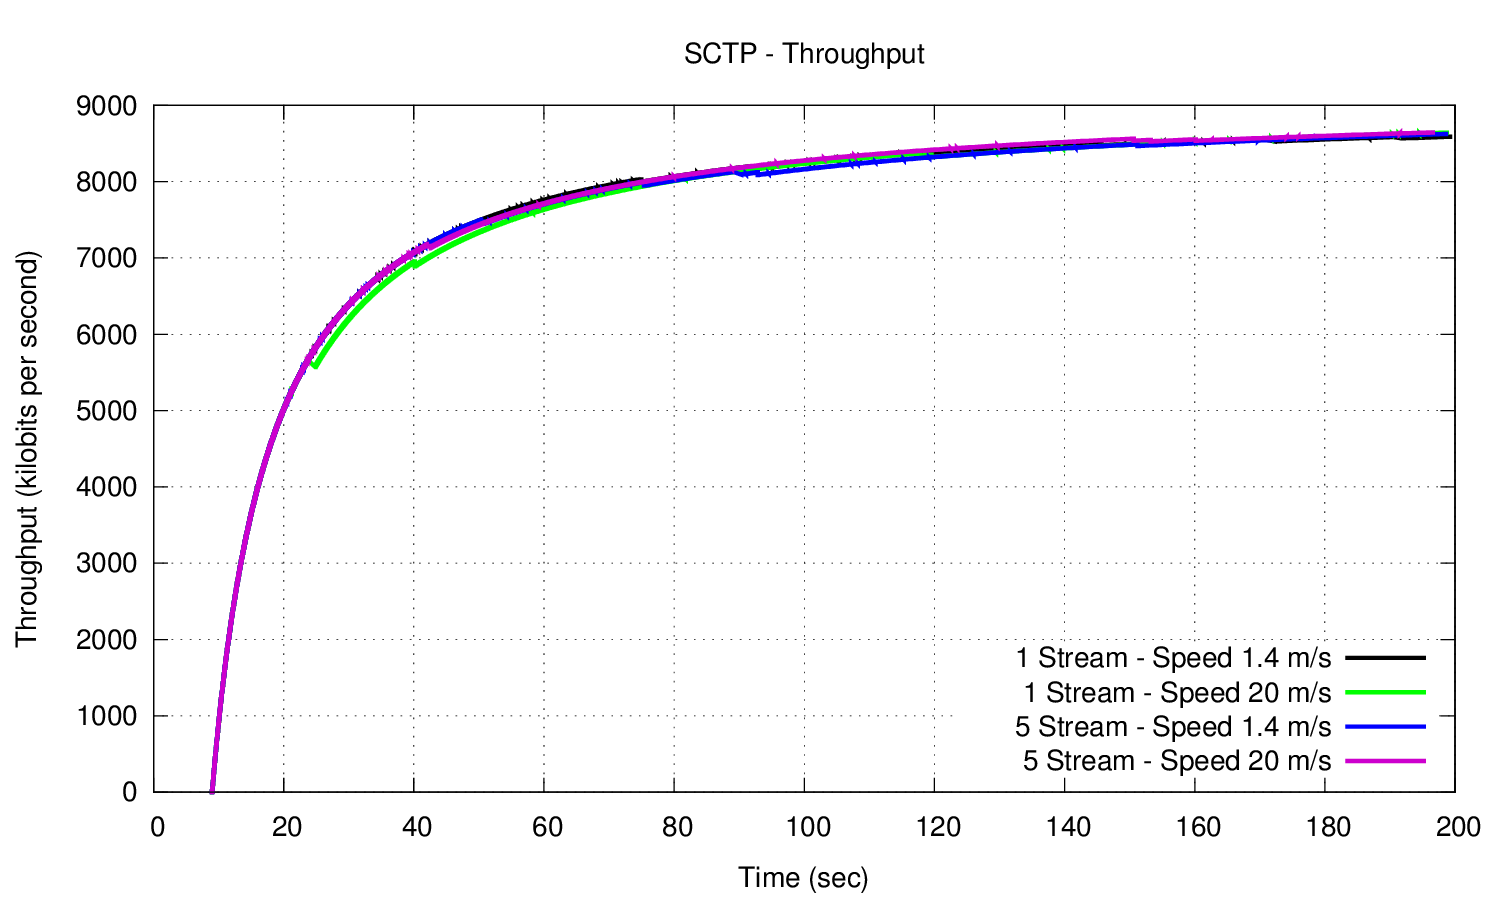
\includegraphics[width=0.8\textwidth]{imgs/sctp-throughput.png}
	\caption{SCTP throughput under varying device movement}
	\label{fig:sctp-throughput}
\end{figure}

Figure \ref{fig:sctp-throughput} shows the throughput over time with 1 and 5 streams and the velocities 1.4 m/s and 20 m/s. Unfortunately the expected performance loss with a higher velocity is not be visible. Independent from the number of streams and the velocity the throughput over time is always in the same range. Because data is transferred it can be assumed that the ad hoc routing is working. Nevertheless it might be possible that the wireless range of the sender and the receiver is enough big that no more hop destinations between are necessary. To validate this assumption the throughput of TCP has been considered.

\begin{figure}[H]
	\centering
	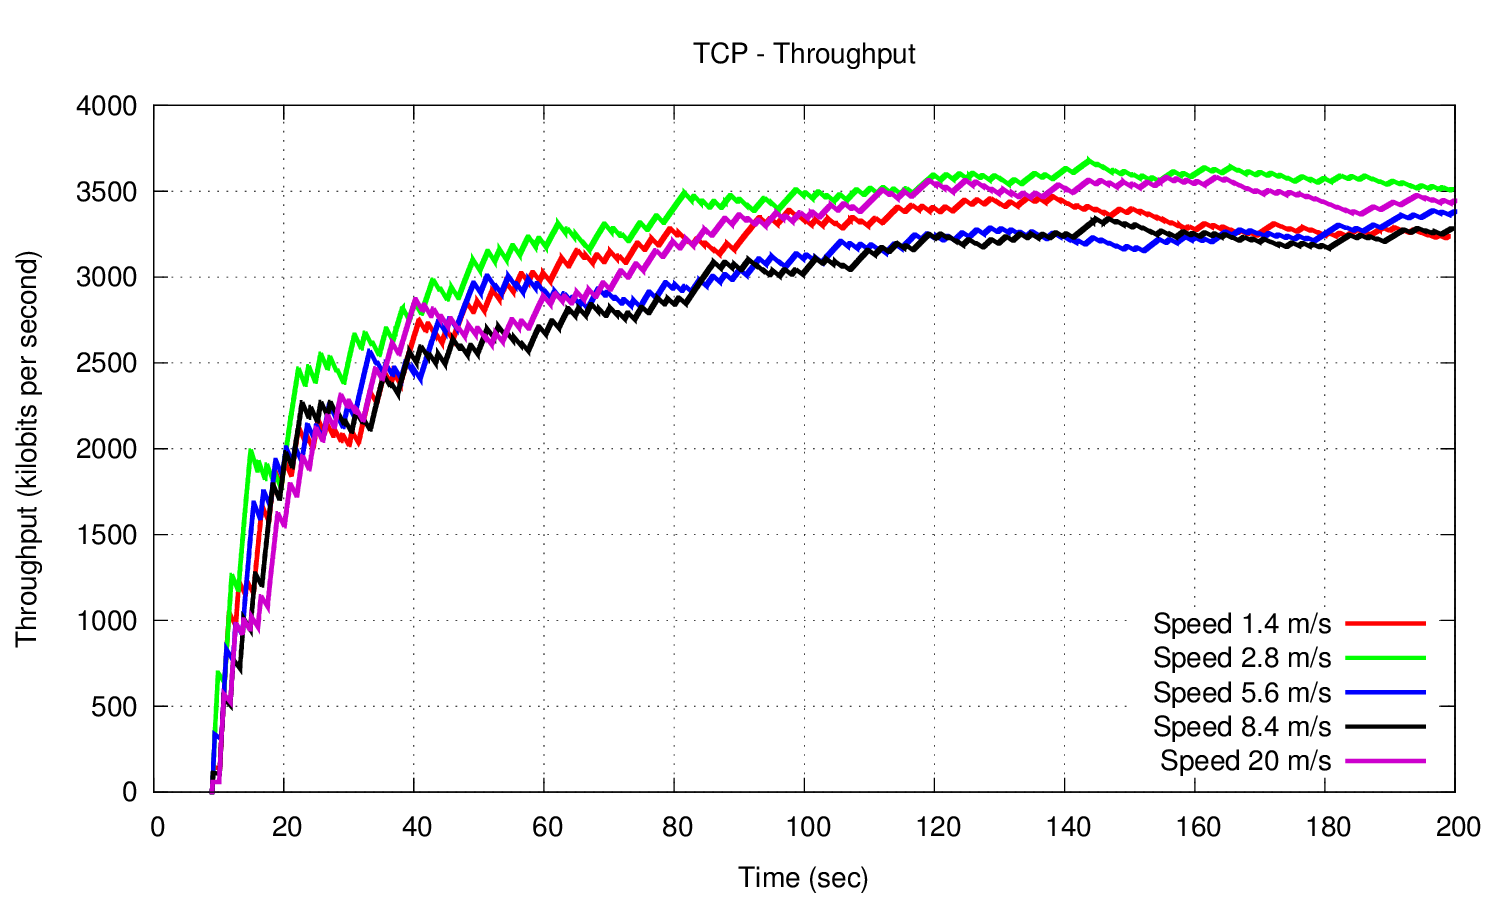
\includegraphics[width=0.8\textwidth]{imgs/tcp-throughput.png}
	\caption{TCP throughput under varying device movement}
	\label{fig:tcp-throughput}
\end{figure}

Figure \ref{fig:tcp-throughput} compares the throughput of the TCP file transfer with different speeds. Like already seen in Figure \ref{fig:sctp-throughput} no direct influence of the increasing velocity can be seen. For example the results of velocity 2.8 and 20 m/s are very close and do not differ significantly like expected. On the basis of these both results the previous announced apprehension that hops between sender and receiver are not use for packet transmission has come true. Modifying the simulation parameters like increasing the path-loss parameter alpha or reducing the maximum transmission power lead to no result because packet transmission was not even possible.

To still be able to discuss the obtained result the velocity parameter will not considered in the following metrics and graphics.

\begin{figure}[H]
	\centering
	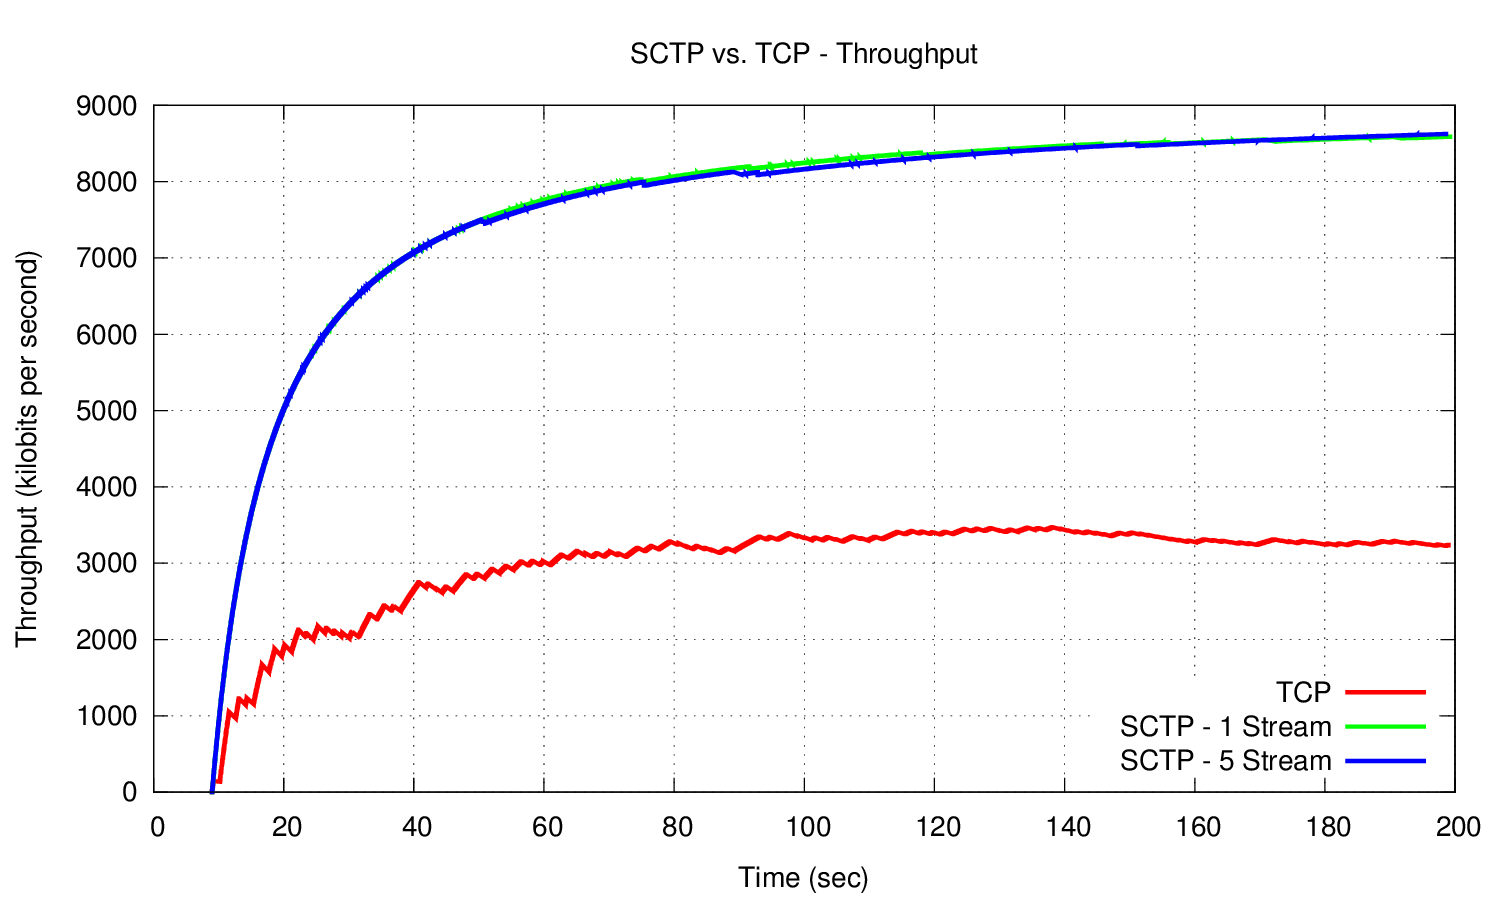
\includegraphics[width=0.8\textwidth]{imgs/sctp-vs-tcp-throughput.png}
	\caption{TCP vs. SCTP throughput}
	\label{fig:tcp-vs-sctp-throughput}
\end{figure}

Figure \ref{fig:tcp-vs-sctp-throughput} compares the throughput of TCP and SCTP over time. It can be seen that independent of the transport protocol the throughput starts growing after about 9 seconds of simulation time. Even thought the file transfer has been initiated at simulation start time this delay exists. A reason for that is the ad hoc routing using the OLSR protocol. While applying this protocol messages can only be forwarded when a corresponding route to the given destination has been found. OLSR needs some time to find neighbours and setup the routing tables. 
Finally when a route has been found data will be sent and the throughput increases with increasing time. In the case of SCTP the throughput increases logarithmic until about the 120 simulation second and then stays constant at the maximum value. In contrast to the smooth curve of SCTP, the throughput increase of TCP is rather erratic. This behaviour is caused by the flow and congestion control mechanisms of the TCP protocol. After about 80 simulation seconds the maximum throughput is reached and stays nearly constant until the end of the simulation.

\paragraph{Round trip time (RTT)}

\paragraph{Loss Rate}

\paragraph{ACK Overhead}

\section{Conclusion}

\begin{thebibliography}{99}
\bibitem {sctp_vs_tcp} SCTP versus TCP: Comparing the Performance of Transport Protocols for Web Traffic, Rajesh Rajamani, Sumit Kumar, Nikhil Gupta, Computer Sciences Department, University of Wisconsin-Madison, July 2002, \url{http://pages.cs.wisc.edu/~sumit/extlinks/sctp.pdf}
\bibitem {sctp_vs_tcp2} A comparison of TCP and SCTP performance using the HTTP protocol, Henrik Osterdahl, \url{http://www.ict.kth.se/courses/IK1550/Sample-papers/Henrik_Oesterdahl-sctp-20050525.pdf}
\bibitem {omnetpp} OMNeT++ Network Simulation Framework, \url{http://www.omnetpp.org/}
\bibitem {sctp_whitepaper} Introduction to the Stream Control Transmission Protocol (SCTP), Paul Stalvig, \url{http://www.f5.com/pdf/white-papers/sctp-introduction-wp.pdf}
\bibitem {aodv_vs_olsr} Comparing AODV and OLSR Routing Protocols, Aleksandr Huhtonen, Helsinki University of Technology, Telecommunication Software and Multimedia Laboratory, \url{http://edge.cs.drexel.edu/regli/Classes/CS680/Papers/Ad%20Hoc/Routing/aodv-oslr-comparison.pdf}
\end{thebibliography}

\end{document}